%% start of file `template.tex'.
%% Copyright 2006-2013 Xavier Danaux (xdanaux@gmail.com).
%
% This work may be distributed and/or modified under the
% conditions of the LaTeX Project Public License version 1.3c,
% available at http://www.latex-project.org/lppl/.


\documentclass[11pt,a4paper,roman]{moderncv}        % possible options include font size ('10pt', '11pt' and '12pt'), paper size ('a4paper', 'letterpaper', 'a5paper', 'legalpaper', 'executivepaper' and 'landscape') and font family ('sans' and 'roman')

% modern themes
\moderncvstyle{banking}                            % style options are 'casual' (default), 'classic', 'oldstyle' and 'banking'
\moderncvcolor{blue}                                % color options 'blue' (default), 'orange', 'green', 'red', 'purple', 'grey' and 'black'
%\renewcommand{\familydefault}{\sfdefault}         % to set the default font; use '\sfdefault' for the default sans serif font, '\rmdefault' for the default roman one, or any tex font name
%\nopagenumbers{}                                  % uncomment to suppress automatic page numbering for CVs longer than one page

% character encoding
\usepackage[utf8]{inputenc}
\usepackage{fontawesome}
\usepackage{tabularx}
\usepackage{ragged2e}
% if you are not using xelatex ou lualatex, replace by the encoding you are using
%\usepackage{CJKutf8}                              % if you need to use CJK to typeset your resume in Chinese, Japanese or Korean

% adjust the page margins
\usepackage[scale=0.8]{geometry}
\usepackage{multicol}
%\setlength{\hintscolumnwidth}{3cm}                % if you want to change the width of the column with the dates
%\setlength{\makecvtitlenamewidth}{10cm}           % for the 'classic' style, if you want to force the width allocated to your name and avoid line breaks. be careful though, the length is normally calculated to avoid any overlap with your personal info; use this at your own typographical risks...

\usepackage{import}

\usepackage{graphicx}
\usepackage{tikz}
\usepackage{tikzpagenodes}
\usetikzlibrary{calc} 
\usepackage[inline]{enumitem}
\usepackage{amsmath}


% personal data
\name{Sajjad P.}{Savoji}
% \title{Curriculum Vitae}                               % optional, remove / comment the line if not wanted
%\address{Gholhak , Tehran , Iran }{}{}% optional, remove / comment the line if not wanted; the "postcode city" and and "country" arguments can be omitted or provided empty
% \phone[mobile]{909-839-3097}                   % optional, remove / comment the line if not wanted
% \phone[fixed]{01234 123456}                    % optional, remove / comment the line if not wanted
%\phone[fax]{+3~(456)~789~012}                      % optional, remove / comment the line if not wanted
% \email{xpan1@swarthmore.edu}                               % optional, remove / comment the line if not wanted
% \homepage{shawnpan.me}                         % optional, remove / comment the line if not wanted
% \extrainfo{}                 % optional, remove / comment the line if not wanted
%\photo[64pt][0.4pt]{picture}                       % optional, remove / comment the line if not wanted; '64pt' is the height the picture must be resized to, 0.4pt is the thickness of the frame around it (put it to 0pt for no frame) and 'picture' is the name of the picture file
%\quote{Some quote}                                 % optional, remove / comment the line if not wanted

% to show numerical labels in the bibliography (default is to show no labels); only useful if you make citations in your resume
%\makeatletter
%\renewcommand*{\bibliographyitemlabel}{\@biblabel{\arabic{enumiv}}}
%\makeatother
%\renewcommand*{\bibliographyitemlabel}{[\arabic{enumiv}]}% CONSIDER REPLACING THE ABOVE BY THIS

% bibliography with mutiple entries
%\usepackage{multibib}
%\newcites{book,misc}{{Books},{Others}}
  
\newcommand*{\customcventry}[7][.25em]{
  \begin{tabular}{@{}l} 
    {\bfseries #4}
  \end{tabular}
  \hfill% move it to the right
  \begin{tabular}{l@{}}
     {\bfseries #5}
  \end{tabular} \\
  \begin{tabular}{@{}l} 
    {\itshape #3}
  \end{tabular}
  \hfill% move it to the right
  \begin{tabular}{l@{}}
     {\itshape #2}
  \end{tabular}
  \ifx&#7&%
  \else{\\%
    \begin{minipage}{\maincolumnwidth}%
      \small#7%
    \end{minipage}}\fi%
  \par\addvspace{#1}}

\newcommand*{\customcvproject}[4][.25em]{
%   \vfill\noindent
  \begin{tabular}{@{}l} 
    {\bfseries #2}
  \end{tabular}
  \hfill% move it to the right
  \begin{tabular}{l@{}}
     {\itshape #3}
  \end{tabular}
  \ifx&#4&%
  \else{\\%
    \begin{minipage}{\maincolumnwidth}%
      \small#4%
    \end{minipage}}\fi%
  \par\addvspace{#1}}

\setlength{\tabcolsep}{12pt}

%----------------------------------------------------------------------------------
%            content
%----------------------------------------------------------------------------------
\begin{document}
	\begin{minipage}[t]{0.2 \textwidth}
		\hspace*{0.4cm}
		\begin{tikzpicture}[baseline=(ola.center),inner sep=0pt]
		\clip (0,0)  circle (2cm) node (ola) {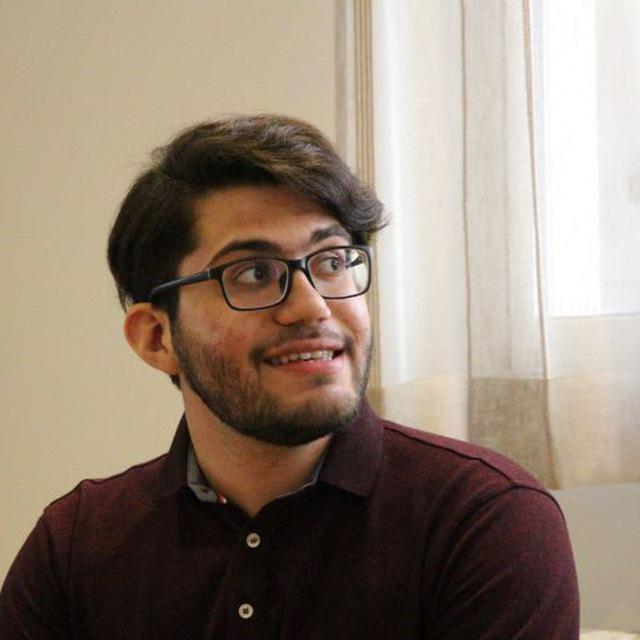
\includegraphics[width=4cm]{resumepic.jpg}};
		\end{tikzpicture}
	\end{minipage}
	\hfill
	\begin{minipage}[t]{0.73\textwidth}
		\makecvtitle
		\vspace*{-23mm}
		\begin{center}
			\begin{tabular}{ c c c }
				 \faEnvelopeO\enspace sj.pakdaman@ut.ac.ir & \faGithub\enspace SajjadPSavoji &  \faMobile\enspace 0098-919-591-9545\\  
			\end{tabular}
			\vspace*{-100mm}
		 Gholhak,Tehran Province,Iran
		\end{center}
	\end{minipage} 
%\begin{CJK*}{UTF8}{gbsn}                          % to typeset your resume in Chinese using CJK
%-----       resume       ---------------------------------------------------------


\section{EDUCATION}
{\customcventry{September 2016 - Present}{Bachelor of Electrical Engineering , Major in Communication Systems , Minor in Computer Engineering}{University of Tehran}{}{}{}}
\begin{itemize}
	\item EE Cumulative GPA: 17.36 / 20
	\item CE Cumulative GPA: 18.13 / 20 	 
\end{itemize}
\subsection{SELECTED COURSES}
	\begin{itemize*}
		\item Artificial Intelligence
		\item Pattern Recognition
		\item Digital Communication Systems
		\item Digital Signal Processing
		\item Communication systems 
		\item Linear Algebra
		\item Statistics and Probability
		\item Operating Systems
		\item Advance Programming
		\item Data Structure
		\item Introduction to Computer Systems and Programming
		\item Linear Control Systems
		\item Linear Control Systems Lab
		\item Digital Logic Design Lab
		\item Realtime Digital Processing Lab
	\end{itemize*}
\section{KEY SKILLS}
	\begin{minipage}[t]{0.5 \textwidth}
		\subsection{Programming Languages}
		\begin{itemize}
			\item C++ (advance)
			\item C (advance)
			\item Python
			\item System Verilog
			\item HTML5 
			\item Java Script
			\item CSS
			\item Bootstrap
		\end{itemize}
	\end{minipage}
	\begin{minipage}[t]{0.5 \textwidth}
		\subsection{Platorms}
		\begin{itemize}
			\item Jupyter notebook and google colaboratory
			\item Matlab simulink \& toolboxes such as FDA-tool
			\item Hardware simulators: Modelsim , Quartus 
			\item Circuit simulators: Multisim
			\item Micro controller simulators: Proteus,Codevision
			\item latex
		\end{itemize}
		\subsection{Micro processors}
		\begin{itemize}
			\item FPGA
			\item DSP
			\item AVR atmeg series
			\item Raspberry Pi 2,3
			\item Arduino
		\end{itemize}
	
	\end{minipage}	

\section{AWARDS AND ACHIEVEMENTS}
\begin{minipage}{\maincolumnwidth}%
	\small{
		\begin{itemize}
			\item $3^{rd}$place in Iran and $93^{th}$ place worldwide in IEEExtreme 11.0 from 2121 teams. participated as team "PointBlank".
			\item $8^{th}$ place in Iran and $733^{th}$ place worldwide in IEEExtreme 12.0 from 3358 teams. participated individually as team "SAVOJI". 
			\item gold medalist basketball player in inter university sport competition festival 2016 and silver medalist in 2017 also gold medalist in inter city of Tehran student sport competition 2014 
			
	\end{itemize}}%
\end{minipage}%

\section{ACADEMIC PROJECTS}

{\customcvproject{AP Drive}{September 2018 - January 2019}
  {\begin{itemize}
    \item A File Hosting Service inspired by Drop Box using C++
    \item Allows multi-user synchronization , file sharing as group and individual , file management,upload and download and storage management for root and admin users. All features are accessible both local and through the net. 
    \item this project was implemented by Object Oriented and multi-file methodology
    \item phase1: Program works similar to linux file system. Implemented locally and without graphical features.
    \item phase2: User interface implementation based on Client-Server distributed model by using web tools.
  \end{itemize}
  }
}

{\customcvproject{Smart House}{Jun 2018 – August 2018}
{\begin{itemize}
  \item IOT based project tested on a wooden home prototype using mostly python and java
  \item By use of a raspberry pi as central gateway of sensor communications , home daily activities such as opening door, powering lights and watering flowers was done automated.
  \item then raspberry interacted through HTTPS and MQTT protocols with a simple android app. as raspberry had massive computation capacity , vital warnings could activate edge computing services such as Fire extinguisher.
  \item all sensors data was stored in thingtalk.ir platform and allowed us to provide user with cloud computing services such as graphs and data conclusions  
\end{itemize}
}

{\customcvproject{Kingdom Rush}{September 2018 - January 2019}
{\begin{itemize}
  \item a real time tower defense game implemented by Simple DirectMedia Layer(SDL) graphical library using C++
  \item the goal of this project was practicing Top-Down design programming methodology
  \item this project was implemented by Object Oriented and multi-file methodology
\end{itemize}
}
}

{\customcvproject{Online Store}{September 2018 - January 2019}
	{\begin{itemize}
			\item modeling a virtual store to manage trades and transactions of goods using C++
			\item this project was implemented by Object Oriented and multi-file methodology
			\item The app provided user with special features such as discount offers , receipts and searching for different features of goods such as price , kind ,etc. 
		\end{itemize}
	}
}

{\customcvproject{git}{October 2016 - November 2016}
	{\begin{itemize}
			\item a simple distributed version-control system for tracking changes in source code during software development which basically works similar to linux git using C 
			\item working with multi dimensional pointers and dynamic memory allocation was the goal of project. 
		\end{itemize}
	}
}
{\customcvproject{Encryption}{June 2017 - July 2017}
	{\begin{itemize}
			\item encrypting short text symbols in color values of pixels using C++
			\item text characters was placed in pixels which had the most variance among it's neighbor pixels  
		\end{itemize}
	}
}
{\customcvproject{Noise removal}{January 2018 - February 2018}
	{\begin{itemize}
			\item removing noise of a .wav file using matlab
			\item first noise was detected and removed by Fourier analysis then using matlab FDA tool a more efficient filter was designed which removed noise perfectly.  
		\end{itemize}
	}
}

{\customcvproject{Frequency Spectrum Analyzer}{January 2019 - February 2019}
	{\begin{itemize}
			\item A real time frequency spectrum analyzer using C and avr atmeg series
			\item Surrounding voice was sampled using avr ADC then using Fast Fourier Transform algorithm , frequency spectrum of voice was shown in a led array.
			\item To assure that hardware was working fine ,sampled data was transmitted to laptop using avr USART and frequency spectrum was double checked in matlab.
		\end{itemize}
	}
}

\section{EXPERIENCE}

{\customcventry{April 2018 - present}{}{Vice Chair of IEEE University of Tehran student branch}{}{}
{\begin{itemize}
  \item The Student Branch Vice-Chair is the junior Executive Officer. He/she should help the Branch Chair with the workload, oversee some of the subcommittees, and manage some of the activities throughout the semester.
\end{itemize}
}

{\customcventry{June - September 2019}{}{Summer Internship in Secure Communication Lab}{University of Tehran}{}
{\begin{itemize}
  \item Secure Communicatin Lab in UofT is a leading lab in which real-life problems is addressed using AI/Deep Learning techniques. Through this reasearch internship I had developed several Artificial Neural Networks such as YOLO2 , LSTM , CNN and MLP. My task was to build a traslator from Iranian Sign Language to written words.  
\end{itemize}
}


{\customcventry{April 2018 - November 2019}{}{IEEExtreme 12.0 and 13.0 ambassador}{International volunteer work}{}
	{\begin{itemize}
			\item IEEEXtreme is an annual hackathon and competitive programming challenge in which teams of IEEE Student members compete in a 24-hour time span against each other to solve a set of programming problems
			\item An ambassador job is to encourage students to participate the challenge
		\end{itemize}
	}	
}
{\customcventry{April 2018 - November 2019}{}{IEEEmadC ambassador}{International volunteer work}{}
	{\begin{itemize}
			\item IEEEmadC (Mobile Applications Development Contest) is an international contest organized by volunteers for IEEE student members across the globe. The main goal is to educate and encourage students to pursue their future career as mobile application developers
			\item An ambassador job is to encourage students to participate the challenge
		\end{itemize}
	}	
}
 \section{MEMBERSHIPS}
 \begin{itemize}
 	
 	\noindent
 	\parbox[t]{.6\textwidth}{\raggedright
 		\item IEEE student member}\hfill
 	\parbox[t]{.1\textwidth}{\centering
 	}\hfill
 	\parbox[t]{.3\textwidth}{\raggedleft
 		September 2017 - present}%
 \end{itemize}


      
}
% Publications from a BibTeX file without multibib
%  for numerical labels: \renewcommand{\bibliographyitemlabel}{\@biblabel{\arabic{enumiv}}}% CONSIDER MERGING WITH PREAMBLE PART
%  to redefine the heading string ("Publications"): \renewcommand{\refname}{Articles}
%\nocite{*}
%\bibliographystyle{plain}
%\bibliography{publications}                        % 'publications' is the name of a BibTeX file

% Publications from a BibTeX file using the multibib package
%\section{Publications}
%\nocitebook{book1,book2}
%\bibliographystylebook{plain}
%\bibliographybook{publications}                   % 'publications' is the name of a BibTeX file
%\nocitemisc{misc1,misc2,misc3}
%\bibliographystylemisc{plain}
%\bibliographymisc{publications}                   % 'publications' is the name of a BibTeX file

%-----       letter       ---------------------------------------------------------

\end{document}


%% end of file `template.tex'.